% !TEX encoding = IsoLatin9
\section{Fonctions r�cursives}
\begin{frame}
  \begin{columns}
    \column{4.8cm}
    \tableofcontents[currentsection,hideothersubsections]
    \column{7cm}
    \centering{
      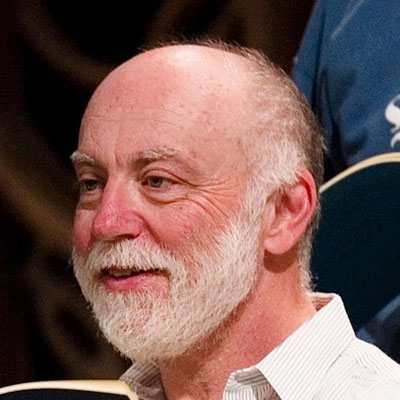
\includegraphics[width=4cm]{fig/deutsch.jpg}
      
      \textit{``To iterate is human, to recurse divine''}\\
      \small{
        \hfill L. Peter Deutsch (1946-)\\
               \hfill auteur de Ghostscript}
    }
  \end{columns}
  
\end{frame}

\begin{frame}[fragile]
\frametitle{Fonction r�cursive}
\begin{block}{}
Un algorithme r�cursif est un algorithme qui, lors
de son ex�cution, s'appelle lui-m�me.
\end{block}
\begin{exampleblock}{Algorithme factorielle}
\begin{algorithmic}[0]
\REQUIRE{n (entier)}\\
\ENSURE{nfact (entier)}\\
\IF {$n=0$}
\RETURN{1}
\ELSE
\RETURN {$n\times$factorielle$(n-1)$}
\ENDIF
\end{algorithmic}
\end{exampleblock}
Le langage C permet la r�cursivit� avec les fonctions :
\begin{codeblock}{}
\vspace{-.3cm}
\lstset{escapeinside={��}}
\lstset{basicstyle=\scriptsize}
\begin{codeC}
int fact (int n) {
  if (n==0) return (1) ;
  else return(n * fact (n-1));
}
\end{codeC}
\vspace{-.3cm}
\end{codeblock}
\end{frame}

\begin{frame}[fragile]
\frametitle{Contexte d'ex�cution}
\begin{block}{}
Chaque appel � la fonction cr�e son propre contexte d'ex�cution
(peut �tre gourmand en m�moire).
\end{block}
\begin{columns}
\column{0.5\textwidth}
\begin{codeblock}{}
\vspace{-.3cm}
\lstset{escapeinside={��}}
\lstset{basicstyle=\scriptsize}
\begin{codeC}
int fact (int n) {
  if (n==0) return (1) ;
  else return(n * fact (n-1));
}

int main() {
  int z ;
  z = fact(4);
}
\end{codeC}
\vspace{-.3cm}
\end{codeblock}

\column{0.4\textwidth}
\begin{figure}
\centering
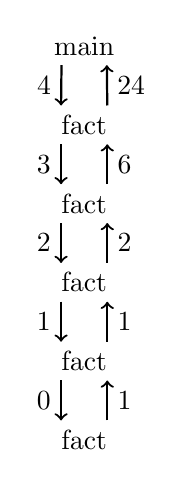
\begin{tikzpicture}[
auto,
node distance=1cm,
]

\node (main) {main} ;
\node (f1) [below of = main] {fact} ;
\node (f2) [below of = f1] {fact} ;
\node (f3) [below of = f2] {fact} ;
\node (f4) [below of = f3] {fact} ;
\node (f5) [below of = f4] {fact} ;

\draw[->,thick] (main.220) -- node [midway, left] {4} (f1.140);
\draw[->,thick] (f1.220) -- node [midway, left] {3} (f2.140);
\draw[->,thick] (f2.220) -- node [midway, left] {2} (f3.140);
\draw[->,thick] (f3.220) -- node [midway, left] {1} (f4.140);
\draw[->,thick] (f4.220) -- node [midway, left] {0} (f5.140);

\draw[->,thick] (f5.40) -- node [midway, right] {1} (f4.320);
\draw[->,thick] (f4.40) -- node [midway, right] {1} (f3.320);
\draw[->,thick] (f3.40) -- node [midway, right] {2} (f2.320);
\draw[->,thick] (f2.40) -- node [midway, right] {6} (f1.320);
\draw[->,thick] (f1.40) -- node [midway, right] {24} (main.320);

\end{tikzpicture}
\end{figure}

\end{columns}

\end{frame}

\begin{frame}
\frametitle{Fonctions r�cursives}
\begin{block}{}
Selon les probl�me trait�s, la r�cursivit� permet
d'obtenir un code source succinct.
\end{block}
Par contre, quand elle est mal r�alis�e :
\begin{itemize}
\item Le code peut tourner sans fin ;
\item La m�moire utilis�e peut �tre �norme (� cause de
la multiplication des contextes d'ex�cution);
\item Cela peut ralentir l'ex�cution du programme.
\end{itemize}
\begin{alertblock}{}
A utiliser avec pr�caution.
\end{alertblock}
\end{frame}